\section{Experiments}
\label{experiment}

In this section, we will introduce datasets and baselines in Section~\ref{Environmental Settings}.
Then, in Section~\ref{Grid World Results}, Section~\ref{Tmaze Results}, Section~\ref{D4RL Results}, and \ref{Ablation}, we report the comparison results, ablation study, and parameters sensitivity analysis. In Appendix~\ref{additional experiments}, we report additional results about offline training time, online testing time, and ablation study.

\subsection{Environmental Settings}
\label{Environmental Settings}
\noindent\textbf{Dataset: Grid World.}~~
We first consider the discrete control environments from the Grid World \cite{14}, which is a commonly used benchmark for recent in-context RL methods. The environments support many tasks that cannot be solved through zero-shot generalization after pre-training because these tasks cannot be inferred easily from the observation. Specifically, we test our method on three environments: Darkroom, Darkroom Hard, and Dark Key-to-Door. In addition, we create a long-term variant of Large Darkroom, Large Darkroom Hard, and Large Darkroom Key-to-Door, where the coordinate space of each environment is expanded to 20 times, and the episode length is expanded 10 times. The dataset is collected from learning histories that are generated by training gradient-based RL algorithms, such as Deep Q-Network \cite{28}. For each environment, we randomly create 60 tasks from the coordinate space and collect data for 1 million steps. 

\noindent\textbf{Dataset: Tmaze.}~~
We also evaluate our method on the Tmaze \cite{19}, a benchmark for testing the recall ability of in-context agents. In Tmaze, any policy that achieves the maximum return must be able to recall information from the first step at the final step. Since the task horizon can be set arbitrarily, it is often used to test the limits of the model's processing of long-term memory.

\noindent\textbf{Dataset: D4RL.}~~
D4RL \cite{13} is a commonly used offline RL benchmark, including continuous control tasks. 
The dataset is collected from Mujoco environments, including HalfCheetah, Hopper, and Walker. The episode length in D4RL is 1000, which is far more than that of Grid World. Therefore, current in-context RL methods require huge computational costs in D4RL, even though it is a commonly used benchmark for conventional RL algorithms.

\noindent\textbf{Baselines.}~~
We investigate the effectiveness and efficiency of DM-H relative to in-context RL, dedicated offline RL, and imitation learning algorithms. Our baselines can be categorized as follows:

\begin{itemize}[noitemsep,leftmargin=*]
\setlist{nolistsep} 
    \item In-context RL: These methods use the transformer to model trajectory sequences and predict actions autoregressively. We compare with recent methods, AMAGO \cite{9}, Decision Pretrained Transformer (DPT) \cite{3}, and Algorithm Distillation (AD) \cite{8}, which achieve impressive results based on the setting of across-episodic contexts.
    % \vspace{-2pt}
    \item Temporal-difference learning: Most temporal-difference (TD) learning methods use an action space constraint or value pessimism and will serve as faithful comparisons to DM-H, representing standard RL methods. Following recent work \cite{1}, we consider state-of-the-art TD3+BC \cite{29} that is demonstrated to be effective on D4RL.
    % \vspace{-2pt}
    \item Imitation learning: Imitation learning methods similarly utilize supervised losses for training, such as Behavior Cloning (BC) \cite{30} and Decision Transformer (DT) \cite{2}. We compare with BC-10$\%$, which is shown to be competitive with state-of-the-art on D4RL. DT also uses a transformer to predict actions autoregressively but is limited to a single episode context.
\end{itemize}

For all comparison methods, we adhere closely to the original hyper-parameter settings. To evaluate DM-H and other in-context RL algorithms, we roll out 10 episodes in D4RL and 20 episodes in Grid World and Tmaze. For each result, we report mean and standard error across 10 random seeds.

\setlength{\belowcaptionskip}{-0.3cm} %调整图片标题与下文距离 
\setlength{\abovecaptionskip}{-0.0cm} %调整图片标题与图距离
\begin{figure*}
    \centering
    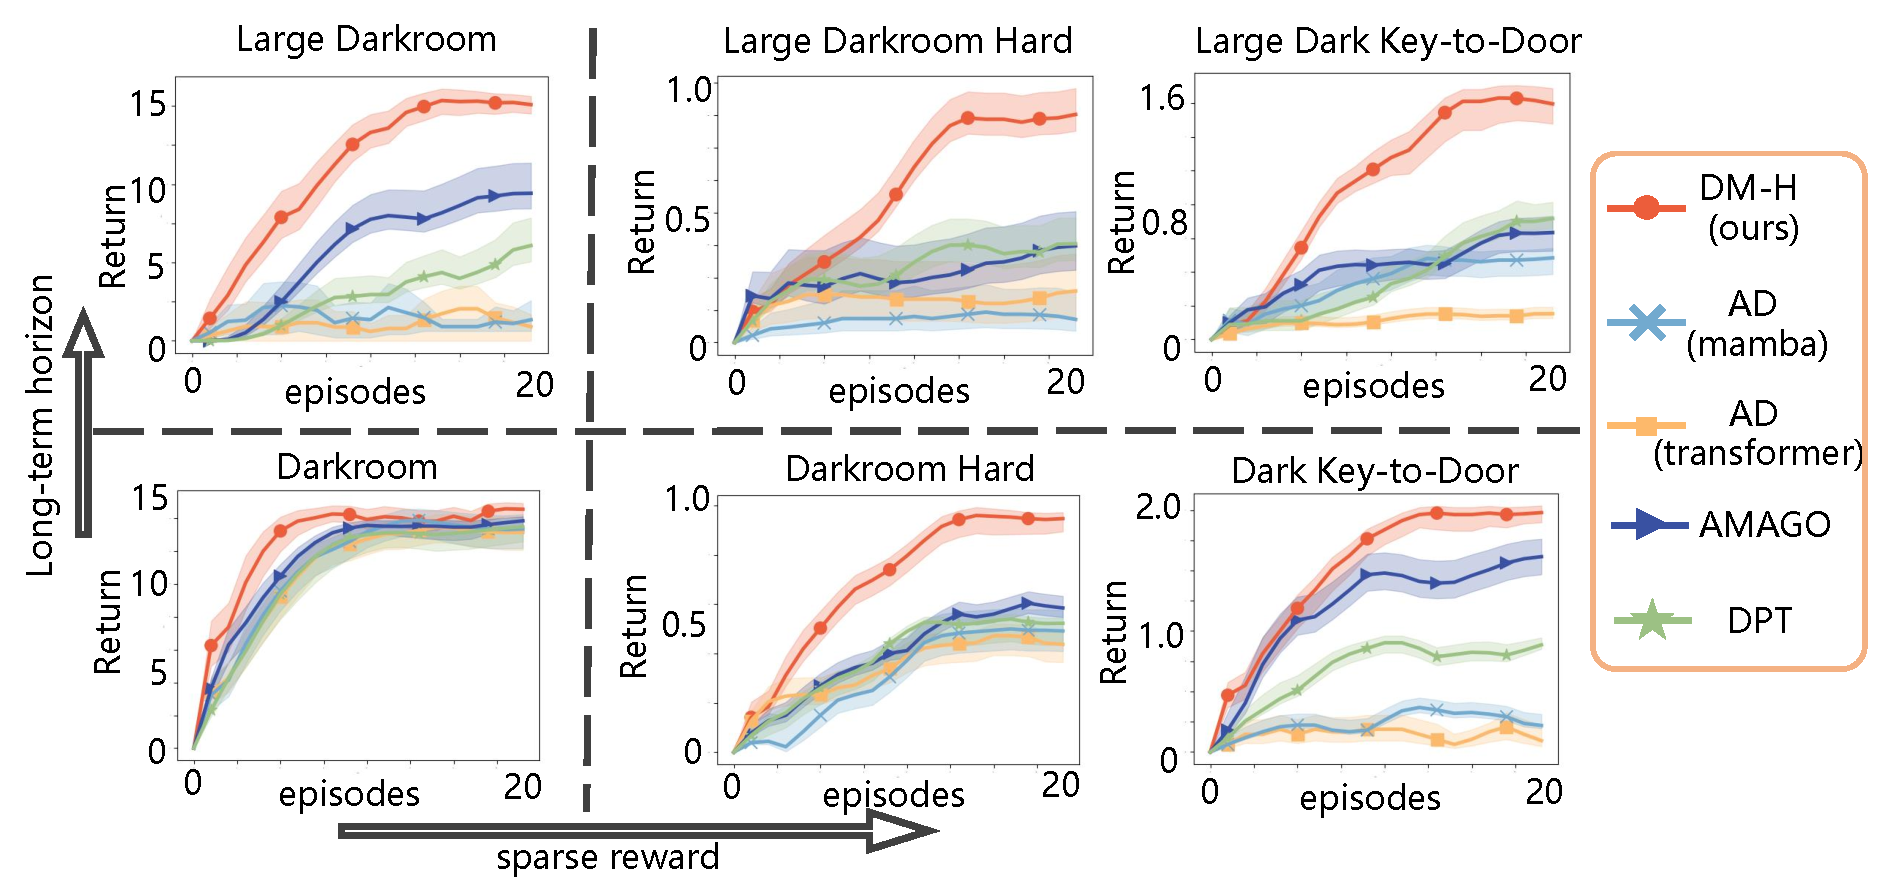
\includegraphics[width=0.9\columnwidth]{Results/maze_results.pdf}
    \caption{Results for Grid World. An agent is expected to solve a new task by interacting with the environments for 20 episodes without online model updates. Our DM-H significantly outperforms baselines on long-term tasks with sparse rewards because it inherits the merits of transformers and Mamba in high-quality prediction and long-term memory.}
    \label{grid world}
\end{figure*}

\subsection{Grid World Results}
\label{Grid World Results}
To evaluate DM-H's self-improvement capabilities in unseen tasks, we compared recent in-context RL methods in the Grid World environments. The agent is required to solve an unseen task by interacting with the environments for 20 episodes without online model updates. In addition, we added a variant of the representative in-context RL AD, replacing the transformer with Mamba as the backbone.

As shown in Figure~\ref{grid world}, DM-H achieves state-of-the-art performance in a wide range of tasks. DM-H achieves 28$\times$ times faster than baselines and more than double the effectiveness as the task horizon increases and rewards become sparse. In long-term tasks, DM-H leverages Mamba's ability to obtain long-term memories while retaining high-quality predictions established by the transformer in decision-making. On the contrary, AD (transformer) and AD (Mamba) only retain one aspect of the advantages of DM-H. In terms of sparse rewards, DM-H is similar to the structure of hierarchical RL, in which Mamba performs a decision every $c$ steps and is, therefore, better at handling reward sparse scenarios. Overall, DM-H demonstrated that the hybrid method is not only feasible but combines more advantages synergetically.

\setlength{\belowcaptionskip}{-0.0cm} %调整图片标题与下文距离 
\setlength{\abovecaptionskip}{-0.0cm} %调整图片标题与图距离
\begin{figure*}
    \centering
    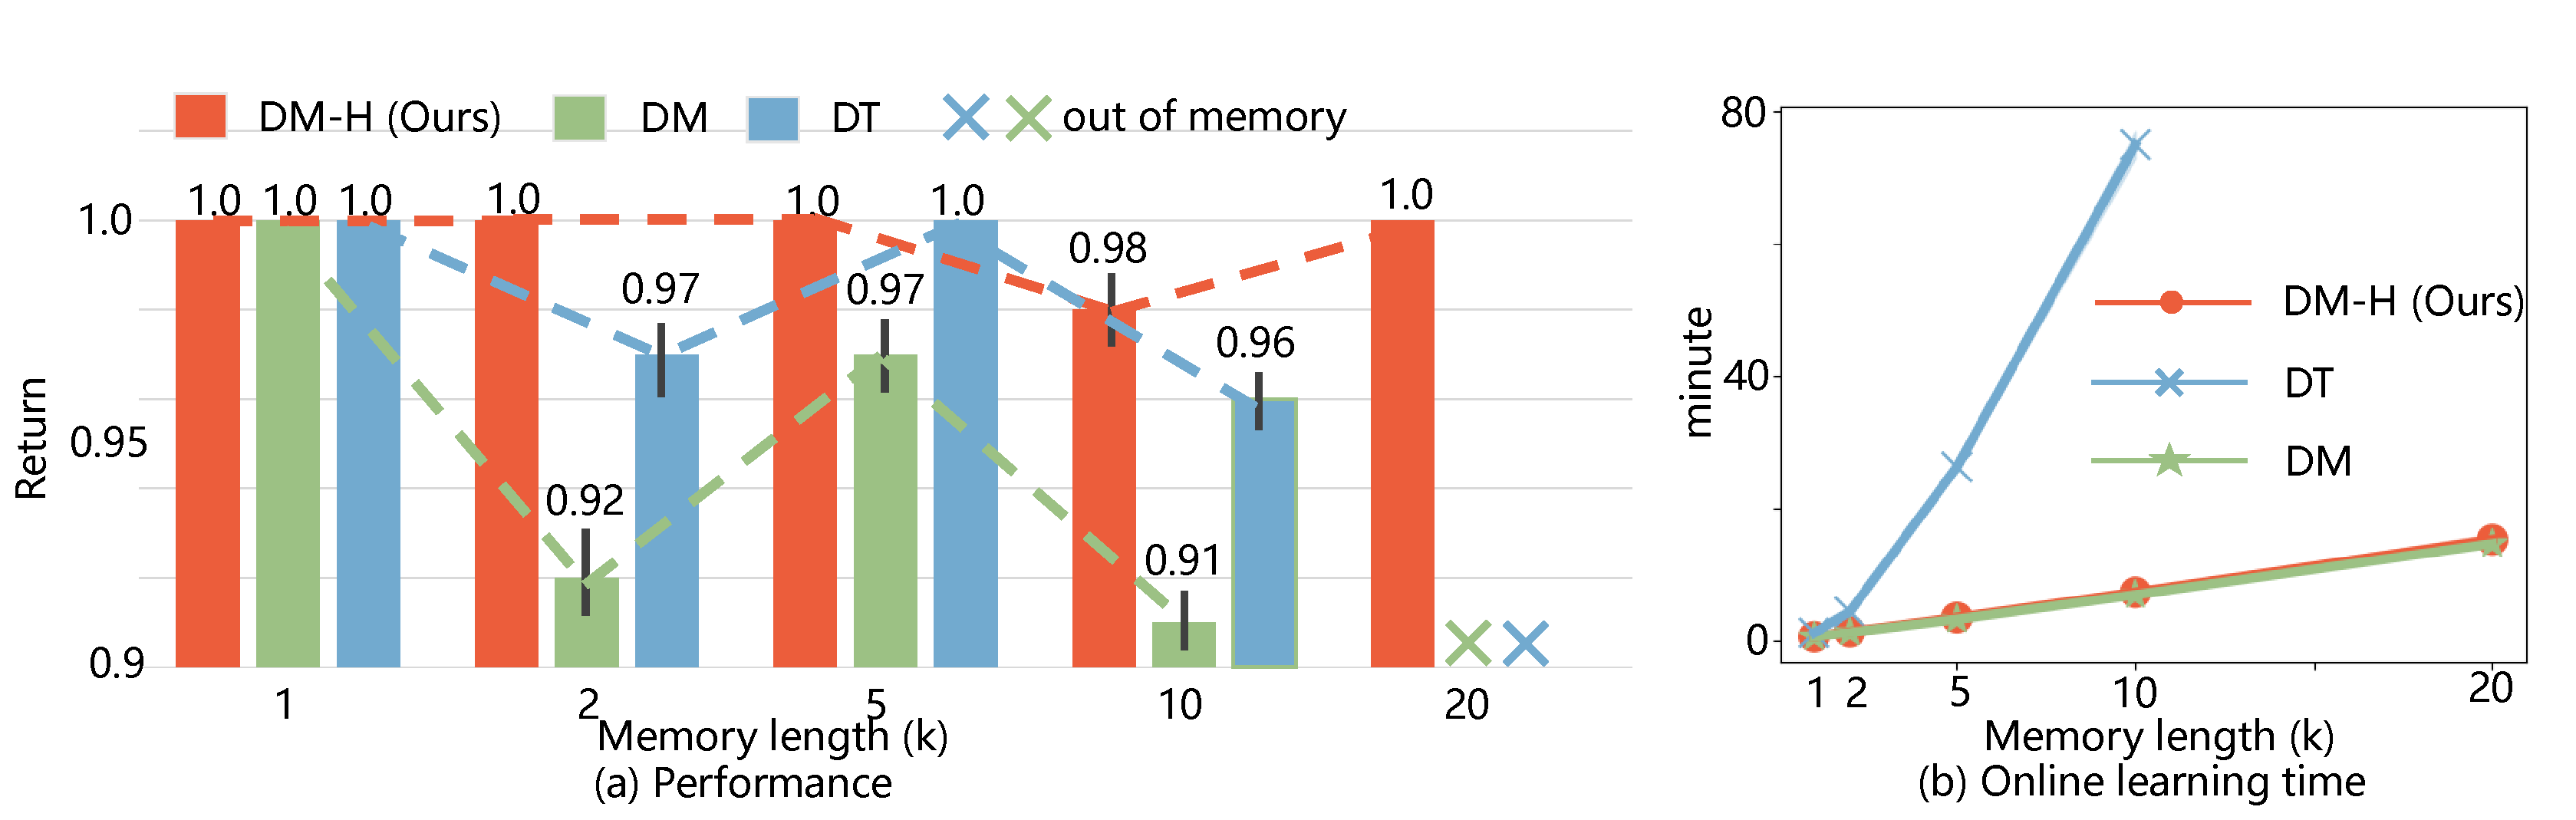
\includegraphics[width=0.95\columnwidth]{Results/Tmaze.pdf}
    \caption{Results for (a) performance and (b) online testing times on Tmaze tasks. We train each method to address Tmaze tasks that have different horizons until we run out of GPU memory at context length to achieve 10k (DT, DM) or 20k (our DM-H). We report the online testing time for 20 episodes of Tmaze tasks.}
    \label{limit}
\end{figure*}

\begin{table*}
\caption{Results for D4RL datasets. DM-H outperforms both in-context RL (DT, AD) and supervised learning (BC) and performs competitively with conventional RL algorithms (TD3+BC and TD3) on almost all tasks.
% The cumulative rewards demonstrate that our SGFD model generalizes well to new values of task-irrelevant features. 
}
\begin{center}
\resizebox{1.0\textwidth}{!}{
\begin{tabular}{lr|rrrrrrr}
\toprule
\specialrule{0em}{1.0pt}{1.0pt}
\toprule
Dataset & Environment & BC-10$\%$ & TD3+BC & TD3 & DT & AD (Mamba) & AD (Transformer) & DM-H \\ 
\toprule
Med-Expert & HalfCheetah & 94.11 & \textbf{96.59} & 87.60 & 93.40 & 92.21\scriptsize{$\pm$ 0.60} & 94.21 \scriptsize{$\pm$ 0.46} & 96.21\scriptsize{$\pm$ 0.28} \\ 
Med-Expert & Hopper & 113.13 & 113.22 & 98.41 & 111.18 & 110.82\scriptsize{$\pm$ 0.56} & 108.32 \scriptsize{$\pm$ 0.95} & \textbf{117.19\scriptsize{$\pm$ 0.65}} \\ 
Med-Expert & Walker2d & 109.90 & 112.21 & 100.52 & 108.71 & 108.31\scriptsize{$\pm$ 0.52} & 111.36 \scriptsize{$\pm$ 0.46}& \textbf{118.21\scriptsize{$\pm$ 0.56}} \\ 
\toprule
Med & HalfCheetah & 43.90 & \textbf{48.93} & 34.60 & 42.73 & 41.92\scriptsize{$\pm$ 0.11} & 42.28 \scriptsize{$\pm$ 1.18} & 45.45\scriptsize{$\pm$ 0.35} \\ 
Med & Hopper & 73.84 & 70.44 & 56.98 & 69.42 & 73.65\scriptsize{$\pm$ 1.23} & 72.58 \scriptsize{$\pm$ 0.54} & \textbf{83.15\scriptsize{$\pm$ 0.63}} \\ 
Med & Walker2d & 82.05 & 86.91 & 70.95 & 74.70 & 78.26\scriptsize{$\pm$ 0.55} &85.96 \scriptsize{$\pm$ 0.46} & \textbf{88.29\scriptsize{$\pm$ 0.76}} \\ 
\toprule
Med-Replay & HalfCheetah & 42.27 & 45.84 & 38.81 & 40.31 & 39.68\scriptsize{$\pm$ 0.13} & 41.28 \scriptsize{$\pm$ 0.21} & \textbf{45.26\scriptsize{$\pm$ 0.43}}\\ 
Med-Replay & Hopper & 90.57 & 98.12 & 78.90 & 88.74 & 82.65\scriptsize{$\pm$ 1.15} &91.32 \scriptsize{$\pm$ 0.66} & \textbf{98.36\scriptsize{$\pm$ 0.51}} \\ 
Med-Replay & Walker2d & 76.09 & 91.17 & 65.94 & 71.22 & 70.92\scriptsize{$\pm$ 1.21} & 89.21 \scriptsize{$\pm$ 1.42}& \textbf{95.66\scriptsize{$\pm$ 1.16}} \\
\toprule
\multicolumn{2}{c|}{Total Average} & 80.65\scriptsize{$\pm$ 1.34} & 84.83\scriptsize{$\pm$ 1.10} & 70.28\scriptsize{$\pm$ 1.20} & 77.69\scriptsize{$\pm$ 1.45} & 76.97\scriptsize{$\pm$ 0.67} & 82.84\scriptsize{$\pm$ 0.70} & \textbf{87.53\scriptsize{$\pm$ 0.59}}\\
\toprule
\specialrule{0em}{1.0pt}{1.0pt}
\toprule
\end{tabular}
}
\end{center}
\label{d4rl}
\end{table*}

\subsection{Tmaze Results}
\label{Tmaze Results}
In this section, we test the limits of DM-H's recall capabilities in the Tmaze task. Solving this task requires accurate recall of the first step at the last step. Therefore, we set the context length equal to the task horizon and compare it with DT and DM, where DM replaces the DT's transformer backbone with a Mamba backbone. We train each method to recover the optimal policy until we run out of GPU memory at a context size equal to 20k (DM-H) or 10k (DT and DM). 

As shown in Figure~\ref{limit}, DM-H achieves the maximum reward with minimum online testing costs at any task horizon, demonstrating that Mamba's recalled memory positively prompts the transformer. Regarding efficiency, DM-H is comparable to DM using only Mamba during online testing and outperforms DM during offline training (Figure~\ref{Tmaze appendix} in Appendix~\ref{additional experiments}). This is because (1) the context of the transformer in DM-H is fixed to the hyperparameter $c$, which does not change with the task length. (2) Mamba model generates a sub-goal every $c$ steps, thereby shortens the sequence it processes by $c\times$ times. Benefiting from these merits, DM-H handles tasks twice the length and has fewer memory resource requirements than DT and DM.

% Compared to DT and DM, DM-H handles twice the length of tasks with fewer memory resources. Regarding effectiveness, DM-H is not inferior to DT in any task horizon. Regarding efficiency, DM-H is comparable to DM using only Mamba.
% This is because (1) the context of the transformer in DM-H is fixed to the hyperparameter $c$, which does not change with the task length. (2) Mamba model generates a sub-goal every $c$ steps, which shortens the sequence it processes by $c\times$ times. As a result, DM-H can handle longer sequences under the same resources and has both high effectiveness and efficiency.

\setlength{\belowcaptionskip}{-0.3cm} %调整图片标题与下文距离 
\setlength{\abovecaptionskip}{-0.0cm} %调整图片标题与图距离
\begin{figure*}
    \centering
    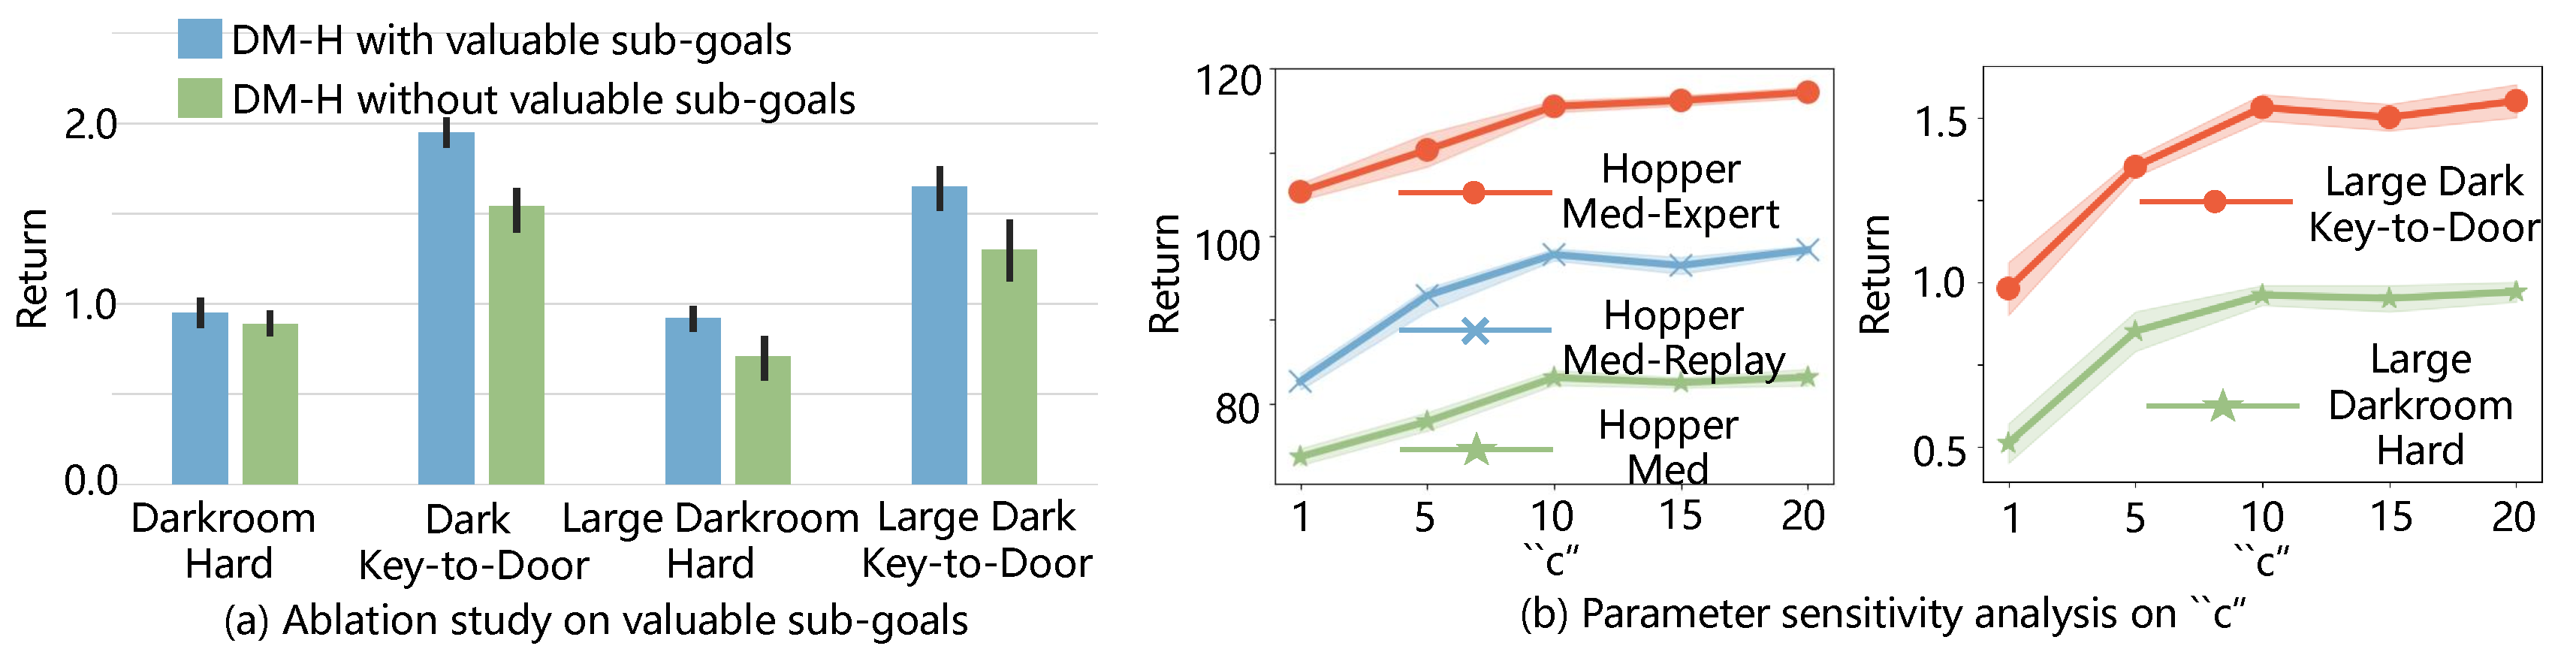
\includegraphics[width=0.9\columnwidth]{Results/Ablation.pdf}
    \caption{(a) The ablation study on DM-H with or without valuable sub-goals. (b) The parameter sensitivity analysis of ``$c$.''}
    \label{ablation}
\end{figure*}

\subsection{D4RL Results}
\label{D4RL Results}
In addition to navigation tasks, we also test DM-H on the control tasks from the D4RL dataset, which is commonly used in conventional offline RL methods. Based on previous work \cite{13}, the results on D4RL are normalized so that 100 denotes an expert policy. Baseline numbers are reported by the Agentic Transformer \cite{1} and from the D4RL paper. As shown in Table~\ref{d4rl}, DM-H outperforms baselines in a majority of the tasks and is competitive with the state-of-the-art in the remaining tasks. In the TD learning and imitation learning categories, TD3+BC is generally the most remarkable algorithm. Compared with them, the superior performance demonstrates the self-improvement of DM-H on suboptimal data.

\subsection{Ablation Study and Parameter Sensitivity Analysis}
\label{Ablation}
\noindent\textbf{Ablation Study on Valuable Sub-goals.}~~
To validate the effectiveness of valuable sub-goals, we conduct an ablation study of DM-H in Grid World tasks.
Figure~\ref{ablation} (a) presents the ablation results, which report the mean episode return across 10 seeds.
We can observe that sub-goals can significantly improve DM-H's performance, proving that the sub-goal strengthens the transformer's dependency on long-term contexts from Mamba. In Appendix~\ref{additional experiments}, we also carry out ablation studies in the D4RL dataset. Please refer to Figure~\ref{appendix ablation}.

\noindent\textbf{Sensitivity of Key Hyperparameters.}~~
In this experiment, we introduce an important hyper-parameter $c$. A large $c$ enables Mamba model to scan multiple episodes with smaller context sizes, significantly improving the computational efficiency. In addition, $c$ also controls the short-term context length in the transformer, which affects the quality of generated actions. As shown in Figure~\ref{ablation} (b), DM-H performs well within the appropriate range of $c$, i.e., $10\leq c \leq 20$.


